\documentclass{beamer}
\usepackage[T1]{fontenc}
\usepackage[utf8]{inputenc}

\usetheme{Madrid}
\usecolortheme{default}
\usepackage{amsmath,amssymb,amsfonts,amsthm}
\usepackage{mathtools}
\usepackage{txfonts}
\usepackage{tkz-euclide}
\usepackage{listings}
\usepackage{adjustbox}
\usepackage{array}
\usepackage{gensymb}
\usepackage{multicol}
\usepackage{gensymb}
\usepackage{tabularx}
\usepackage{gvv}
\usepackage{lmodern}
\usepackage{circuitikz}
\usepackage{tikz}
\lstset{literate={·}{{$\cdot$}}1 {λ}{{$\lambda$}}1 {→}{{$\to$}}1}
\usepackage{graphicx}

\setbeamertemplate{page number in head/foot}[totalframenumber]

\usepackage{tcolorbox}
\tcbuselibrary{minted,breakable,xparse,skins}



\definecolor{bg}{gray}{0.95}
\DeclareTCBListing{mintedbox}{O{}m!O{}}{%
  breakable=true,
  listing engine=minted,
  listing only,
  minted language=#2,
  minted style=default,
  minted options={%
    linenos,
    gobble=0,
    breaklines=true,
    breakafter=,,
    fontsize=\small,
    numbersep=8pt,
    #1},
  boxsep=0pt,
  left skip=0pt,
  right skip=0pt,
  left=25pt,
  right=0pt,
  top=3pt,
  bottom=3pt,
  arc=5pt,
  leftrule=0pt,
  rightrule=0pt,
  bottomrule=2pt,
  toprule=2pt,
  colback=bg,
  colframe=orange!70,
  enhanced,
  overlay={%
    \begin{tcbclipinterior}
    \fill[orange!20!white] (frame.south west) rectangle ([xshift=20pt]frame.north west);
    \end{tcbclipinterior}},
  #3,
}
\lstset{
    language=C,
    basicstyle=\ttfamily\small,
    keywordstyle=\color{blue},
    stringstyle=\color{orange},
    commentstyle=\color{green!60!black},
    numbers=left,
    numberstyle=\tiny\color{gray},
    breaklines=true,
    showstringspaces=false,
}
\title{9.4.22}
\subtitle{Quadratic with equal roots}
\author{EE25BTECH11010 - Arsh Dhoke}
\date{}
\begin{document}

\frame{\titlepage}

\begin{frame}{Question}
Find the value of $k$ such that the quadratic equation
$
kx(x-2) + 6 = 0
$
has equal roots. Verify your solution using graph.
\end{frame}

\begin{frame}{Solution}
\begin{align}
kx^2 - 2kx + 6 = 0
\end{align}
This can be represented as a conic:
\begin{align}
\vec{x}^{T}\vec{V}\vec{x} + 2\vec{u}^{T}\vec{x} + f = 0
\end{align}
where
\begin{align}
\vec{V} = \myvec{k & 0 \\ 0 & 0}, \quad
\vec{u} = \myvec{-k \\ 0}, \quad
f = 6
\end{align}
\end{frame}

\begin{frame}{Condition for Equal Roots}
For the roots of the quadratic to be equal, the line $y=0$ (the $x$-axis)
must be tangent to the conic.
The condition for tangency of a line $\vec{n}^{T}\vec{x} = c$ with a conic
$\vec{x}^{T}\vec{V}\vec{x} + 2\vec{u}^{T}\vec{x} + f = 0$ is:
\begin{align}
\vec{u}^{T}\vec{V}^{-1}\vec{u} - f = 0
\end{align}
For the given conic:
\begin{align}
\vec{V}^{-1} = \myvec{\frac{1}{k} & 0 \\ 0 & 0}
\end{align}
\end{frame}

\begin{frame}{Finding $k$}
\begin{align}
\vec{u}^{T}\vec{V}^{-1}\vec{u} - f &= 0 \\
\implies
\myvec{-k & 0}
\myvec{\frac{1}{k} & 0 \\ 0 & 0}
\myvec{-k \\ 0} - 6 &= 0 
\end{align}
$
\therefore k = 6
$
Thus, the quadratic becomes:
$
6x^2 - 12x + 6 = 0
$
or equivalently,
$
(x - 1)^2 = 0
$
which clearly has a double root at $x = 1$.
\end{frame}

\begin{frame}{Verification by Graph}
\begin{figure}[ht!]
\centering
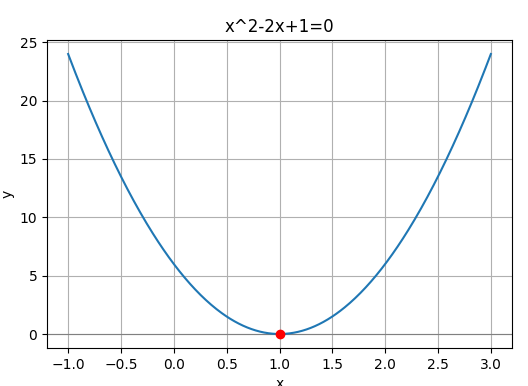
\includegraphics[height=0.6\textheight, keepaspectratio]{figs/parabola.png}
\caption{Graph of $y = 6x^2 - 12x + 6$ showing a double root at $x=1$}
\end{figure}
\end{frame}

\begin{frame}[fragile]
    \frametitle{C Code}
\begin{lstlisting}
#include <math.h>

double find_k() {
    double k1, k2;     
    double a, b, c;    
    double D;          

    // Equation: 4k^2 - 24k = 0
    a = 4;
    b = -24;
    c = 0;
    D = b * b - 4 * a * c;

    k1 = (-b + sqrt(D)) / (2 * a);
    k2 = (-b - sqrt(D)) / (2 * a);

\end{lstlisting}
\end{frame}

\begin{frame}[fragile]
    \frametitle{C Code}
\begin{lstlisting}
    // k = 0 or 6, but k = 0 makes equation invalid
    if (k1 != 0)
        return k1;
    else
        return k2;
}

\end{lstlisting}
\end{frame}


\begin{frame}[fragile]
    \frametitle{Python Code}
\begin{lstlisting}
import numpy as np
import matplotlib.pyplot as plt

k = 6
x = np.linspace(-1, 3, 400)
y = k*x*(x-2) + 6   # kx^2 - 2kx + 6

plt.figure(figsize=(6,4))
plt.axhline(0, color='gray', linewidth=0.8)
plt.plot(x, y, label=f'k={k} : y=kx(x-2)+6')
plt.scatter([1], [0], color='red', zorder=5)   # double root at x=1
plt.title('x^2-2x+1=0')
plt.xlabel('x')
plt.ylabel('y')
plt.grid(True)
plt.savefig("/home/arsh-dhoke/ee1030-2025/ee25btech11010/matgeo/9.4.22/figs/parabola.png")
plt.show()

\end{lstlisting}
\end{frame}

\begin{frame}[fragile]
    \frametitle{Python+ C Code}
\begin{lstlisting}
import ctypes
import numpy as np
import matplotlib.pyplot as plt

# Load the shared C library
lib = ctypes.CDLL("./code.so")

# Define the return type of the C function
lib.find_k.restype = ctypes.c_double

# Call the C function
k = lib.find_k()
print("Value of k for equal roots:", k)

# Define the quadratic function
def f(x, k):
    return k * x * (x - 2) + 6
\end{lstlisting}
\end{frame}

\begin{frame}[fragile]
    \frametitle{Python+ C Code}
\begin{lstlisting}
# Create x values
x = np.linspace(-1, 3, 200)
y = f(x, k)

# Plot the quadratic
plt.plot(x, y, label=f"k = {k:.2f}")
plt.axhline(0, color="black", linewidth=0.8)  # x-axis
plt.axvline(0, color="black", linewidth=0.8)  # y-axis
plt.title("Quadratic: kx(x - 2) + 6 = 0 (Equal Roots Condition)")
plt.xlabel("x")
plt.ylabel("y")
plt.legend()
plt.grid(True)
plt.savefig("/home/arsh-dhoke/ee1030-2025/ee25btech11010/matgeo/9.4.22/figs/parabola.png")
plt.show()

\end{lstlisting}
\end{frame}
\end{document}
